\documentclass[11pt,a4paper]{article}

\usepackage[utf8]{inputenc}
\usepackage[T1]{fontenc}
\usepackage[ngerman]{babel}
\usepackage[a4paper,margin=2.5cm]{geometry}
\usepackage{graphicx}
\usepackage{booktabs}
\usepackage{tabularx}
\usepackage{longtable}
\usepackage{array}
\usepackage{float}
\usepackage{microtype}
\usepackage[hidelinks]{hyperref}
\usepackage{enumitem}
\usepackage{caption}
\usepackage{xurl}

\setlist{nosep,leftmargin=*}
\setlength{\parindent}{0pt}
\setlength{\parskip}{0.55em}
\captionsetup{font=small,labelfont=bf}
\graphicspath{{../daten/img/}{../modelle/img/}}

\title{Meilenstein 1:\\Problemverständnis, Data Understanding und Baseline}
\author{Domänenprojekt 2 -- Kultur- und Entwicklungsstadiumsklassifikation\\[0.5em]
Team: \AE-R\O\O T\\
Mitglieder: Achim Duong, Pascal Heinzemann, Jan-David Wiederstein}
\date{Stand: 06.10.2026\\Code-Version: \textit{[Commit oder Branch ergänzen]}}

\begin{document}
\maketitle

\section{Domäne und Ziel}

\subsection{Fachlicher Kontext}

Die Aufgabenbeschreibung behandelt satellitengestützte Hyperspektralaufnahmen landwirtschaftlicher
Flächen in den USA. EO-1 Hyperion erfasst Reflexion in vielen schmalen Spektralkanälen von
ungefähr 10\,nm Breite. Die Aufgabenfolien beschreiben jede Beobachtung als ein Feld und nennen
eine räumliche Auflösung von 30\,m. Im bereitgestellten Datensatz entspricht eine Zeile einem
Spektrum; ob jede Zeile unverändert genau einem Originalpixel entspricht, ist anhand der
Tabellendaten allein nicht nachprüfbar.

Neben den Spektralbändern enthält der Datensatz \texttt{AEZ} und \texttt{Month}. Laut
Aufgabenbeschreibung fassen agroökologische Zonen Gebiete mit ähnlichen natürlichen
Anbaubedingungen zusammen, unter anderem Klima, Böden und Vegetationsperiode. Diese Angaben
sind möglicher zusätzlicher Kontext für die Klassifikation; ihre Verfügbarkeit und Aussagekraft
für spätere, neue Daten muss bei der Bewertung berücksichtigt werden.

\subsection{Projektziel und fachliche Relevanz}

Das Projektziel ist die zuverlässige Klassifikation der Kulturpflanze (\texttt{Crop}) und ihres
Entwicklungsstadiums (\texttt{Stage}) anhand der spektralen Signaturen aus EO-1-Hyperion-Aufnahmen.
Die Aufgabenbeschreibung formuliert den Zielansatz hierarchisch: zuerst die Kulturpflanzenart,
dann das Entwicklungsstadium innerhalb der vorhergesagten Kulturklasse. Andere Strategien --
beispielsweise kombinierte Crop-Stage-Klassen oder getrennte Modelle -- sind ebenfalls zulässig,
sofern sie begründet und miteinander verglichen werden.

Die Aufgabenbeschreibung begründet die Relevanz mit der landwirtschaftlichen Bestandsaufnahme,
der Planung von Bewirtschaftungsmaßnahmen sowie der Erstellung präziserer Modelle, Karten und
Überwachungsmöglichkeiten. Satellitenbeobachtungen können eine großflächige Klassifikation
ermöglichen, ohne jeden Standort einzeln aufsuchen zu müssen. Das Projekt prüft die
Klassifikationsleistung auf den bereitgestellten Daten; es weist nicht nach, dass eine konkrete
Bewirtschaftungsentscheidung dadurch verbessert wird.

\subsection{Untersuchungs- und Bewertungsziel}

Neben der Entwicklung eines Klassifikators verlangt die Aufgabenbeschreibung den Vergleich
unterschiedlicher Modellierungsstrategien und die Untersuchung, ob sich die Eingabedaten durch
Dimensionsreduktion verringern lassen, ohne die Klassifikationsleistung zu verschlechtern.
Bewertet werden sowohl \texttt{Crop} als auch \texttt{Stage}. Wegen der ungleichen
Klassenverteilung nennt die Aufgabenbeschreibung Balanced Accuracy und Macro-F1 als zentrale
Metriken; Sample-F1 ist eine weitere Projektmetrik. Ergebnisse sollen für beide Zielgrößen und
mit Blick auf die Klassenverteilung interpretiert werden.

\section{Data Understanding}

\subsection{Umfang und Merkmale}

\begin{table}[htbp]
\centering
\caption{Umfang und verfügbare Merkmale der Datensätze}
\begin{tabularx}{\textwidth}{l r l X}
\toprule
Datensatz & Beobachtungen & Zielwerte & Eingaben \\
\midrule
Training & 5.591 & \texttt{Crop}, \texttt{Stage} & Spektralbänder, \texttt{AEZ}, \texttt{Month} \\
Test & 1.397 & nicht vorhanden & Spektralbänder, \texttt{AEZ}, \texttt{Month} \\
\bottomrule
\end{tabularx}
\end{table}

Die Tabelle enthält 198 Spektralspalten mit Wellenlängen von 427 bis 2.395\,nm. In beiden
Datensätzen sind dieselben 67 Bänder vollständig leer; 131 Bänder enthalten Messwerte. In sechs
weiteren verfügbaren Bändern fehlen einzelne Werte, insgesamt sind davon 44 Trainings- und 11
Testzeilen betroffen.

\subsection{Labelverteilung und spektrale Muster}

Die Labels sind unausgewogen: \texttt{rice} umfasst 93 Trainingsbeobachtungen, gegenüber 2.097
bei \texttt{corn}; \texttt{Harvest} ist mit 180 Beobachtungen das seltenste Stadium, während
\texttt{Critical} mit 1.541 am häufigsten vorkommt. Bei den Crop--Stage-Paaren reicht die
Häufigkeit von 11 Beobachtungen für \texttt{cotton} $\times$ \texttt{Harvest} bis 675 für
\texttt{corn} $\times$ \texttt{Critical}. Insgesamt kommen 23 der 30 möglichen Kombinationen
im Training vor. Die nicht beobachteten Kombinationen sind ein Befund zur Stichprobe und
belegen nicht, dass diese Kombinationen fachlich unmöglich sind.

\begin{figure}[htbp]
\centering
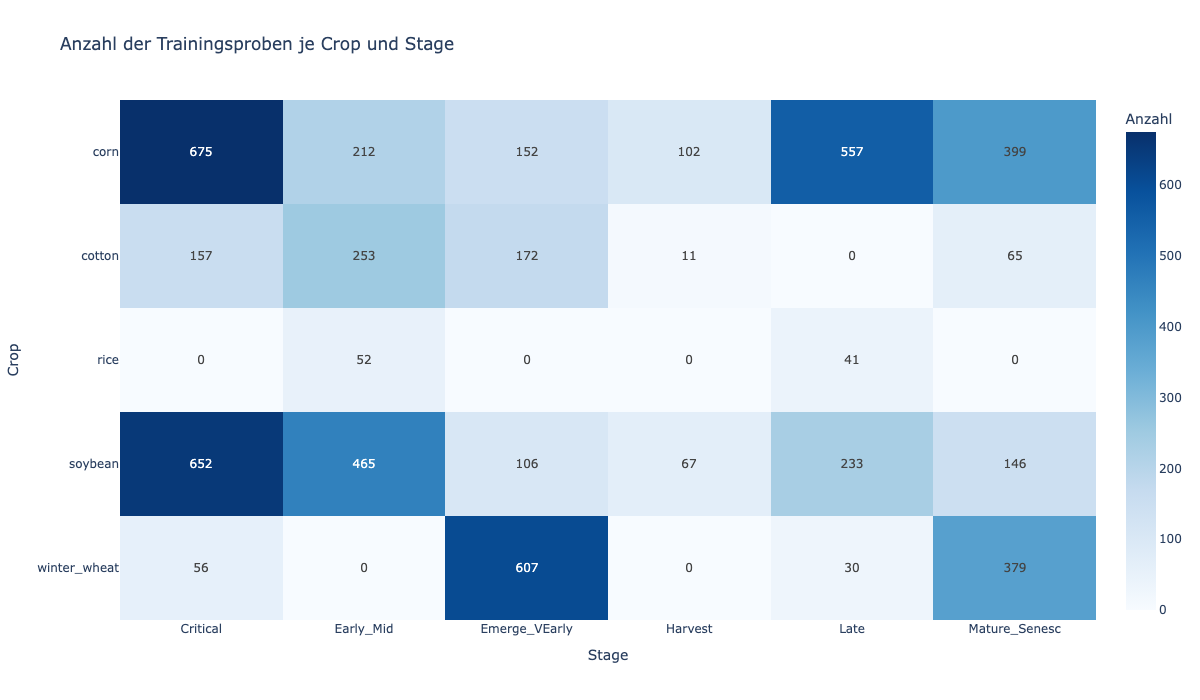
\includegraphics[width=0.92\textwidth]{../daten/img/EDA_anzahl_der_trainingsproben_je_crop_und_stage.png}
\caption{Häufigkeit der beobachteten Crop-Stage-Kombinationen.}
\end{figure}

Die mittleren Spektren unterscheiden sich zwischen Kulturen und teilweise zwischen Stadien
innerhalb einer Kultur. Die Streuung und Überlappung zwischen Gruppen bleibt sichtbar; die
Spektren trennen die Zielklassen daher nicht vollständig. Benachbarte verfügbare Bänder sind
stark korreliert. \texttt{AEZ} und \texttt{Month} hängen ebenfalls mit der Labelverteilung
zusammen. Beispielsweise ist \texttt{Month} 8 bei \texttt{corn} im Training nur mit
\texttt{Critical} vertreten. Diese Muster motivieren Modellvarianten, belegen aber keine
Vorhersageleistung.

\begin{figure}[htbp]
\centering
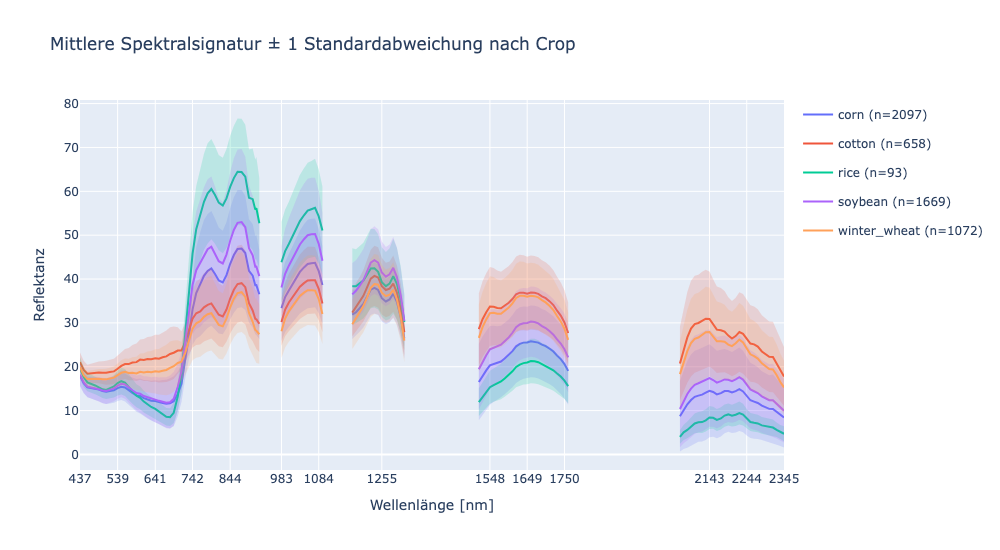
\includegraphics[width=0.96\textwidth]{../daten/img/EDA_mittlere_spektralsignatur_1_standardabweichung_nach_crop.png}
\caption{Mittlere Spektralsignaturen nach Crop; Unterschiede und Überlappungen zeigen, wie
trennbar die Kulturen anhand der Spektren erscheinen.}
\end{figure}

\begin{figure}[htbp]
\centering
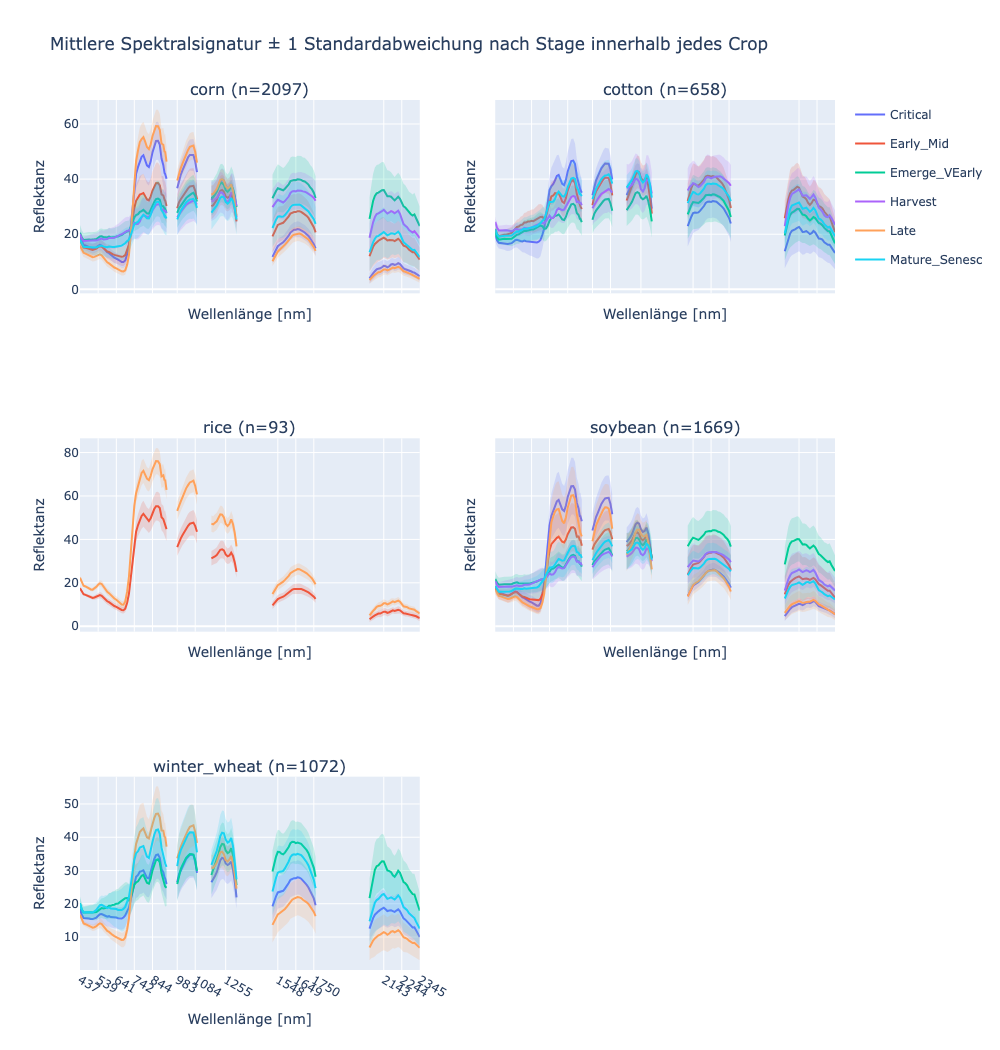
\includegraphics[width=0.96\textwidth]{../daten/img/EDA_mittlere_spektralsignatur_1_standardabweichung_nach_stage_innerhalb_jedes_crop.png}
\caption{Mittlere Stadien-Spektren innerhalb jeder Crop-Klasse; Streuung und Überlappung
veranschaulichen die Schwierigkeit der Stage-Vorhersage.}
\end{figure}

\begin{figure}[htbp]
\centering
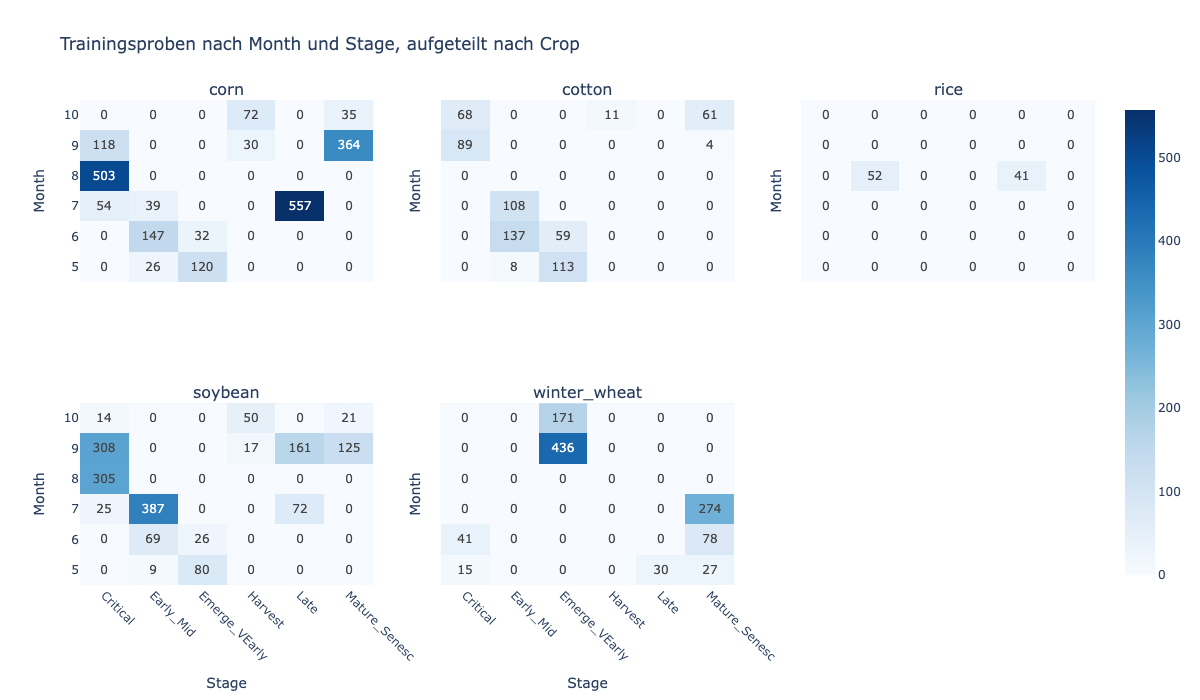
\includegraphics[width=0.96\textwidth]{../daten/img/EDA_trainingsproben_nach_month_und_stage_aufgeteilt_nach_crop.png}
\caption{Stage-Häufigkeiten nach Month innerhalb jeder Crop-Klasse; die Verteilung zeigt den
Zusammenhang zwischen Kontextmerkmalen und Labels.}
\end{figure}

\subsection{Datenqualität, Ausreißer und Ähnlichkeit}

Im Training wurden zwei Paare identischer Eingaben mit übereinstimmenden Labels gefunden.
Zwischen vollständigen Train- und Test-Spektren der verfügbaren Bänder wurden keine exakten
Treffer festgestellt. Der explorative Similarity-Screen fand innerhalb derselben
Crop-Stage-Gruppe viele Paare mit hoher Cosinus-Ähnlichkeit. Da die verwendete Schwelle nicht
als Duplikatgrenze validiert ist und Feld- oder Aufnahme-IDs fehlen, belegt das weder Duplikate
noch gemeinsame Flächen oder Leakage.

Die Ausreißer- und Sprungdiagnostik markiert Kandidaten zur Prüfung, bestätigt aber keine
fehlerhaften Messungen. Insbesondere die verfügbaren Bänder \texttt{X912}, \texttt{X915} und
\texttt{X923} werden nicht allein wegen ihrer Lage oder eines lokalen Kurvenverlaufs entfernt.
Eine technische oder biologische Ursache der dortigen Auffälligkeiten ist anhand der
vorliegenden Angaben nicht belegt.

\subsection{Grenzen der Datengrundlage}

Feld-, Bild- oder räumliche Gruppenkennungen liegen in der verwendeten Tabelle nicht vor.
Deshalb lässt sich nicht feststellen, ob ähnlich erscheinende Spektren abhängige Beobachtungen
sind. Auch die technische Ursache vollständig leerer Bänder und die genaue Vorverarbeitung vor
Bereitstellung des Datensatzes sind nicht abschließend dokumentiert. Die mögliche
Übertragbarkeit auf andere Regionen, Jahre oder Aufnahmebedingungen wird mit diesem
Holdout-Split nicht belegt.

\section{Erste Data-Preprocessing-Pipeline}

\subsection{Pipeline-Ablauf}

\textit{[Wird von der zuständigen Person ergänzt.]}

\subsection{Cleaning- und Preprocessing-Entscheidungen}

Die folgenden Empfehlungen stützen sich auf die explorative Datenanalyse. Sie unterscheiden
zwischen unmittelbar begründeten Bereinigungen und Varianten, deren Nutzen erst in einer
sauberen Validierung geprüft werden muss.

\begingroup
\small
\setlength{\tabcolsep}{3pt}
\renewcommand{\arraystretch}{1.15}
\begin{longtable}{p{2.4cm}p{6.0cm}p{7.0cm}}
\caption{Cleaning- und Preprocessing-Empfehlungen aus der EDA.}\label{tab:cleaning-entscheidungen}\\
\toprule
Thema & Empfehlung & Begründung \\
\midrule
\endfirsthead
\toprule
Thema & Empfehlung & Begründung \\
\midrule
\endhead
\midrule
\multicolumn{3}{r}{Fortsetzung auf der nächsten Seite}\\
\endfoot
\bottomrule
\endlastfoot

Vollständig leere Bänder & Die 67 vollständig leeren Bänder aus den Modellmerkmalen entfernen; die 131 verfügbaren zunächst als Rohband-Baseline behalten. & Leere Spalten enthalten keine Messinformation. Die Ursache ihres Fehlens ist nicht belegt. Die verfügbaren Bänder \texttt{X912}, \texttt{X915} und \texttt{X923} nicht allein wegen ihrer Nähe zu leeren Bändern entfernen. \\

Fehlende Einzelwerte & Verbleibende Lücken innerhalb eines Spektrums interpolieren und Randlücken mit dem nächstgelegenen vorhandenen Wert behandeln. Die Imputation innerhalb der Modellpipeline durchführen. & Es fehlen einzelne Bandwerte in wenigen Zeilen. Die Vorverarbeitung muss innerhalb jedes Trainingsfolds angepasst werden, damit keine Validierungsinformation einfließt. \\

Glättung & Keine Glättung als Standard-Cleaning einführen. Falls begründet, wenige vorab festgelegte Varianten als eigene Modellvarianten in der Cross-Validation vergleichen (Meilenstein 2). & Lokale Sprung- oder Unruhekandidaten belegen keinen allgemeinen Glättungsbedarf. Glättung könnte auch informative spektrale Unterschiede abschwächen. \\

Ausreißer & Isolation-Forest- und klassenweise Mahalanobis-Scores zum Markieren und Prüfen verwenden; Zeilen nicht allein aufgrund eines Scores automatisch löschen. & Ein hoher Score beweist keinen Messfehler. Besonders Mahalanobis-Abstände sind bei vielen Bändern und kleinen Crop-Stage-Gruppen vorsichtig zu interpretieren. \\

Exakte Duplikate & Die zwei identischen Trainingspaare vor dem Split deduplizieren, sofern die Labels übereinstimmen. Near-Duplicates nicht anhand eines frei gewählten Schwellenwerts löschen. & Exakte Wiederholungen könnten sonst auf verschiedene Split-Teile geraten. Spektralähnlichkeit allein beweist weder fehlerhafte Daten noch dieselbe Beobachtungsquelle. \\

Ähnliche Spektren / Leakage & Ähnlichkeit als Prüfhypothese dokumentieren. Falls Feld-, Bild- oder Aufnahme-IDs verfügbar sind, abhängige Beobachtungen gemeinsam splitten. & Innerhalb einer Klasse zeigen ähnliche Spektren zunächst mögliche Redundanz. Abhängige Messungen auf beiden Seiten der Split-Grenze könnten die Evaluation optimistisch machen; die vorhandenen Daten belegen eine solche Abhängigkeit nicht. \\

Split und Evaluation & Den kombinierten Crop-Stage-Label beim stratifizierten Split berücksichtigen und Cross-Validation nur auf dem Trainingsanteil durchführen. Balanced Accuracy und Macro-F1 jeweils für Crop und Stage berichten. & Die Klassen sind unausgewogen und das kleinste beobachtete Paar umfasst 11 Zeilen. Stratifizierung hilft, seltene Paare zu erhalten, garantiert aber keine räumlich unabhängige Evaluation. \\

\texttt{AEZ} und \texttt{Month} & Varianten mit und ohne Kontextmerkmale vergleichen. & Die Merkmale hängen mit der Labelverteilung zusammen; ihre Verfügbarkeit und Stabilität beim späteren Einsatz sind gesondert zu klären. \\
\end{longtable}
\endgroup

\section{Erster Baseline-Klassifikator}

\subsection{70/30 Clusterplot-Split}

\textit{[Tatsächlich verwendete Split-Methode und Klärung des Begriffs
„Clusterplot-Split“ ergänzen.]}

\subsection{Modell und Code}

\textit{[Modell, Merkmale, Einstellungen und Code-Einstiegspunkt ergänzen.]}

\subsection{Kurzer Demo-Run}

\textit{[Ausführungsbefehl, Demo-Ablauf und erzeugte Ausgabe ergänzen.]}

\subsection{Ergebnisse und kurze Einordnung}

\textit{[Metriken für Crop und Stage, Vergleichsreferenz und wichtigste Beobachtungen
ergänzen.]}

\section{Fazit, offene Punkte und nächste Schritte}

\subsection{Ergebnis von Meilenstein 1}

\begin{itemize}
  \item Domänenziel und Grenzen der Vorhersage sind beschrieben.
  \item Datenumfang, Labelungleichgewicht, fehlende Bänder und sichtbare spektrale
        Überlappungen wurden untersucht.
  \item Pipeline und Baseline werden in den dafür vorgesehenen Abschnitten dokumentiert.
\end{itemize}

\subsection{Offene Punkte}

\begin{itemize}
  \item Bedeutung des geforderten „70/30 Clusterplot-Splits“ klären.
  \item Verfügbarkeit von Feld-, Bild- oder räumlichen IDs sowie die Bedeutung von
        \texttt{Month} und \texttt{AEZ} klären.
  \item Herkunft und Vorverarbeitung der Spektralbänder klären.
\end{itemize}

\subsection{Nächste Schritte}

\begin{itemize}
  \item Die Pipeline- und Baseline-Abschnitte nach den jeweiligen Demo-Läufen vervollständigen.
  \item Modelle mit und ohne \texttt{AEZ} und \texttt{Month} sowie begründete Glättungs- oder
        Merkmalsreduktionsvarianten innerhalb derselben Cross-Validation vergleichen.
\end{itemize}

\section{Quellen im Projekt}

\begin{itemize}
  \item Domänenbeschreibung: \url{../domaene/index.md}
  \item Data Understanding und EDA: \url{../daten/m1-data-understanding.md}
  \item Vollständige EDA-Dokumentation: \url{../daten/eda.md}
  \item Datenpipeline: \url{../daten/pipeline.md}
  \item Baseline-Ergebnisse: \url{../modelle/ansaetze/baseline.md}
  \item Offene Fragen an die Betreuung: \url{offene-fragen.md}
\end{itemize}

\end{document}
